\documentclass{vgtc}                         % final (conference style)
%\documentclass[review]{vgtc}                  % review
%\documentclass[widereview]{vgtc}             % wide-spaced review
%\documentclass[preprint]{vgtc}               % preprint
%\documentclass[electronic]{vgtc}             % electronic version
\let\ifpdf\relax
% Included Packages
\usepackage{fancyhdr}
\usepackage[labelfont=bf,textfont=it]{caption}
\usepackage{verbatim}
\usepackage{color}
\usepackage{listings}
\usepackage{amsfonts}
\usepackage{multirow}
\usepackage{amssymb,amsmath}
\usepackage{mathptmx}
\usepackage{graphicx}
\usepackage{times}
\usepackage{algorithm}
\usepackage{algpseudocode}

\usepackage{url}
\usepackage{xcolor}
% \renewcommand{\algorithmiccomment}[1]{// #1}

% \definecolor{bluekeywords}{rgb}{0.13,0.13,1}
% \definecolor{greencomments}{rgb}{0,0.5,0}
% % \definecolor{redstrings}{rgb}{0.9,0,0}
% \definecolor{gray}{rgb}{0.4,0.4,0.4}
% \definecolor{darkblue}{rgb}{0.0,0.0,0.6}
% \definecolor{cyan}{rgb}{0.0,0.6,0.6}
% % \definecolor{softwhite}{rgb}{0.98,0.98,0.98}

% \definecolor{redstrings}{gray}{0.4}

% \definecolor{softwhite}{gray}{0.95}

% \definecolor{darkblue}{gray}{0.6}

% \definecolor{bluekeywords}{gray}{0.6}

% \definecolor{gray}{gray}{0.6}

% \definecolor{cyan}{gray}{0.7}

% \definecolor{greencomments}{gray}{0.5}



\lstset{
breaklines=true,
float, 
mathescape=true, 
texcl=true,
basicstyle=\footnotesize\ttfamily,
columns=fixed,
numbers=none,
emph={normalize,mul,stars,voronoi}
stepnumber=1,
captionpos=b,
showstringspaces=true,
language=C++,
keywordstyle=\color[rgb]{0.0, 0.0, 0.8},
stringstyle=\color[rgb]{0.5, 0.0, 0.5},
tabsize=4,
commentstyle=\color[rgb]{0.133,0.545,0.133}\textit,
morekeywords={float3,float4,float2},
frame=single,
escapeinside={(*@}{@*)} 
}

%% If you are submitting a paper to a conference for review with a double
%% blind reviewing process, please replace the value ``0'' below with your
%% OnlineID. Otherwise, you may safely leave it at ``0''.
\onlineid{0}

%% declare the category of your paper, only shown in review mode
\vgtccategory{Research}

%% allow for this line if you want the electronic option to work properly
\vgtcinsertpkg

%% In preprint mode you may define your own headline.
%\preprinttext{To appear in an IEEE VGTC sponsored conference.}

%% Paper title.

\title{Procedural Celestial Rendering for 3D Navigation}

\author{
Alain Galvan\thanks{e-mail:agalvan@fiu.edu} \and
Francisco Ortega\thanks{e-mail:fortega@fiu.edu} \and
Naphtali Rishe\thanks{e-mail:ndr@acm.org}
}
\affiliation{School of Computing and Information Sciences \\ Florida International University}

\teaser{
  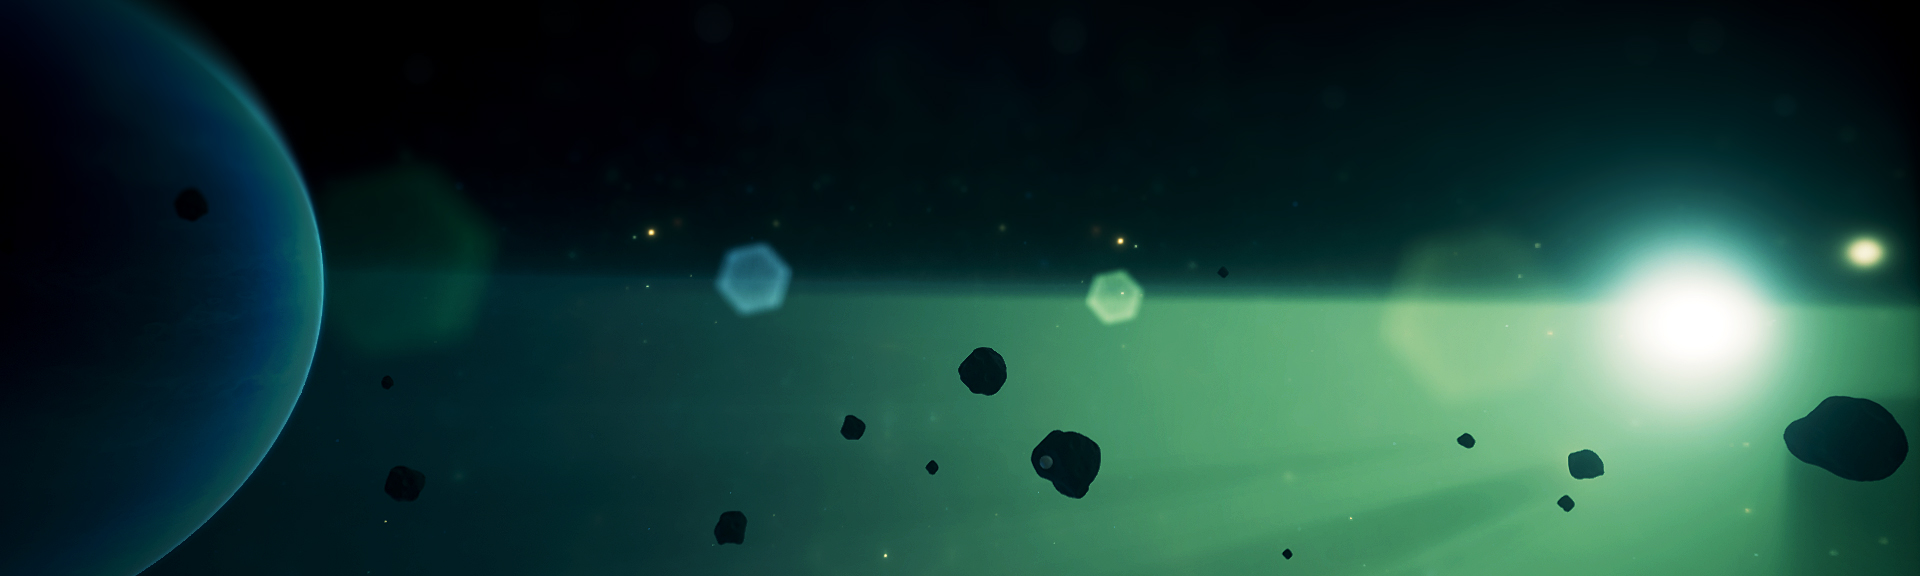
\includegraphics[width=\textwidth]{../images/cover.jpg}
  \caption{An example 3D environment using our method of skybox generation. }
}

%% Abstract section.
\abstract{
   Finding the best suitable environment for 3D navigation that utilizes at least six degrees-of-freedom is still difficult. Furthermore, creating a system to procedurally generate a large virtual environment provides an opportunity for researchers to understand this problem further. Therefore, we present a novel  technique to render a parametric celestial skybox with the ability to light environments similar to natural color corrected images from telescopes. We first pre-compute a spherical ray map that corresponds to the cubemap coordinates, then generate stars and dust through a combination of different noise generation shaders. 

} % end of abstract

\keywords{natural phenomena, 3d navigation, physically-based rendering, image-based lighting}


%% ACM Computing Classification System (CCS). 
%% See <http://www.acm.org/class/1998/> for details.
%% The ``\CCScat'' command takes four arguments.

\CCScatlist{ 
  \CCScat{I.3.7}{Three-Dimensional Graphics and Realism}%
{Color, shading, shadowing, and texture}{Fractals};
  \CCScat{H.5.2}{User Interfaces}{3D Navigation}{User Interaction}
}

%% Copyright space is enabled by default as required by guidelines.
%% It is disabled by the 'review' option or via the following command:
% \nocopyrightspace

%%%%%%%%%%%%%%%%%%%%%%%%%%%%%%%%%%%%%%%%%%%%%%%%%%%%%%%%%%%%%%%%
%%%%%%%%%%%%%%%%%%%%%% START OF THE PAPER %%%%%%%%%%%%%%%%%%%%%%
%%%%%%%%%%%%%%%%%%%%%%%%%%%%%%%%%%%%%%%%%%%%%%%%%%%%%%%%%%%%%%%%%

\begin{document}

%% The ``\maketitle'' command must be the first command after the
%% ``\begin{document}'' command. It prepares and prints the title block.

%% the only exception to this rule is the \firstsection command
\firstsection{Introduction}

\maketitle

%% \section{Introduction} 

3D navigation is an important pillar of user interaction. Navigation includes travel (the engine that takes us from point A to point B) and wayfinding (our cognitive spatial understanding of the environment)~\cite{Bowman:2004vo}. 3D travel may include six degrees-of-freedom (DOF) depending on the domain requirements; however, in many instances, a user may require less than 6 DOF. This leads to a question on what type of environment is best suited to test 6-DOF interactions (translations and rotations on the x,y, and z axes)? We believe that the cosmos provides such environment to derive generic gestures (or actions) that may serve in other 3D visualization environments. The primary reason for this observation is that users may find it necessary to perform all the translations and rotations for this environment. 

This paper presents one approach that may allow other researchers to easily create large sets of data for interaction studies. This will be valuable to the 3D User Interfaces (3DUI) community. Instead of manually creating spaces, there are methods to automate this process (see Section \ref{sec:relatedwork}). We propose a newer method that provides an efficient real-time algorithm to render celestial skies as the problem of large expanses of space still poses a problem for real-time rendering. For example, some common techniques include the use of pseudo-random noise clamped to specific intervals or the use of static measured data. However, these techniques fail to accurately represent space or fail to offer parametric control. %%%


\section{Related Work}
\label{sec:relatedwork}


There has been plenty of research in rendering physically-accurate day and night skies, but ambient light from stars and space has not been given much attention. For Final Fantasy XV, Elcott et al. attempted a similar technique of procedurally generating a sky with raymarching, but used light probes rather than an ambient cubemap to apply lighting effects to the environment~\cite{Elcott:2016geba}. Limberger et al. attempted to render stars using billboards that are processed with a pixel shader to adjust their brightness and color~\cite{Limberger:2012}.

Jensen et al. provided a model for physically accurate night skies but opted to use measured data to diffuse galactic and cosmic light~\cite{Jensen:2001fr}. They enumerated sources of night illumination that we've opted to use in this paper, namely diffuse galactic/cosmic light. Elek and Kmoch provided a model for spectral scattering  but focused on the effect this had on planetary atmospheres~\cite{Elek:t+B4baGRba}. Similarly, other researchers have focused on a physically accurate atmospheric scattering model~\cite{Bruneton:2008id,Haber:2005hl}. We make use of the technique Bruneton and Neyret provided for planetary bodies in our example, but opt to focus on outer space~\cite{Bruneton:2008id}.

Our approach uses a cubemap (a 3D texture consisting of 6 faces), which has been used as a fast way of providing ambient lighting for mobile devices, and has been by shown by Trindade et al. to also serve in the use of rendering multi-scale 3D navigation environments~\cite{Trindade:2011}.


\section{Approach}


We first formulate a physically-based model for starlight and stardust based on the user's origin position, star size, and temperature. We combine this with volumetric raymarching (a volumetric form of ray-casting) techniques for clouds and dust. The model is applied via a shader (see Listing \ref{lst:shader}) to generate a high-dynamic range cubemap. The result of the cubemap is a real-time, efficient, and realistic environment that can be used either as a background, a reflection map, or an ambient cubemap light source. What is most interesting about our approach is that if we applied our technique to a ambient cubemap, a more rich animated interface would be created because of the described dynamic lighting. 

\begin{lstlisting}[caption={Fragment Shader for Celestial Rendering}, label={lst:shader}, float]

float3 rayDirection = $\textbf{normalize}$(mul(uniforms.ViewMatrix, float4(UV-float2(0.5, 0.5), .5, 0.))).xyz;

OutColor.a = 1.0;
OutColor.rgb = $\textbf{stars}$(rayDirection, uniforms.elapsedTime);
OutColor.rgb += $\textbf{voronoi}$(rayDirection, uniforms.elapsedTime);

\end{lstlisting}

Algorithm \ref{alg:HighLevelStars} works by processing a cubemap render target. A cube based spherical directional map is generated by the shader, as shown in Figure \ref{fig:cubemap}, which is then used as an input to a four dimensional noise generation algorithm based on the work of Perlin et al. to create volumetric diffuse effects~\cite{Perlin:2002}. The output of the noise generation algorithms is composited with a white noise function mapped to sharp changes in luminosity values. We utilized Varonoi noise because Zaninetti observed that the distribution of galaxies in the universe closely resembles Voronoi diagrams~\cite{Zaninetti:2013fa}.  Finally, due to the intense processing power required to render an entire cubemap for every frame, we employ update throttling and dynamically change the skybox resolution. Our system is implemented as a plugin for Unreal Engine 4. Our source code is easy to use and requires minimal changes to existing scenes. It is currently available for download at \url{https://github.com/OpenHID/realtime-celestial-rendering}. 



\begin{algorithm}[tbh]                      % enter the algorithm environment
	\caption{General Algorithm For Celestial Rendering}          % give the algorithm a caption
	\label{alg:HighLevelStars}                           % and a label for \ref{} commands later in the document
	\begin{algorithmic}[1]                    % enter the algorithmic environment
    \Ensure all input/output buffers must have been initialized
%%    \REQUIRE Calibration and T = 1/FS
	\For{$cubeFace = 1$ to $6$}
	\State {$runShader(Texture[cubeFace],RotationMatrix[cubeFace])$}
	\EndFor	
	\end{algorithmic}
\end{algorithm}
\begin{figure}[ht]
  \centering
  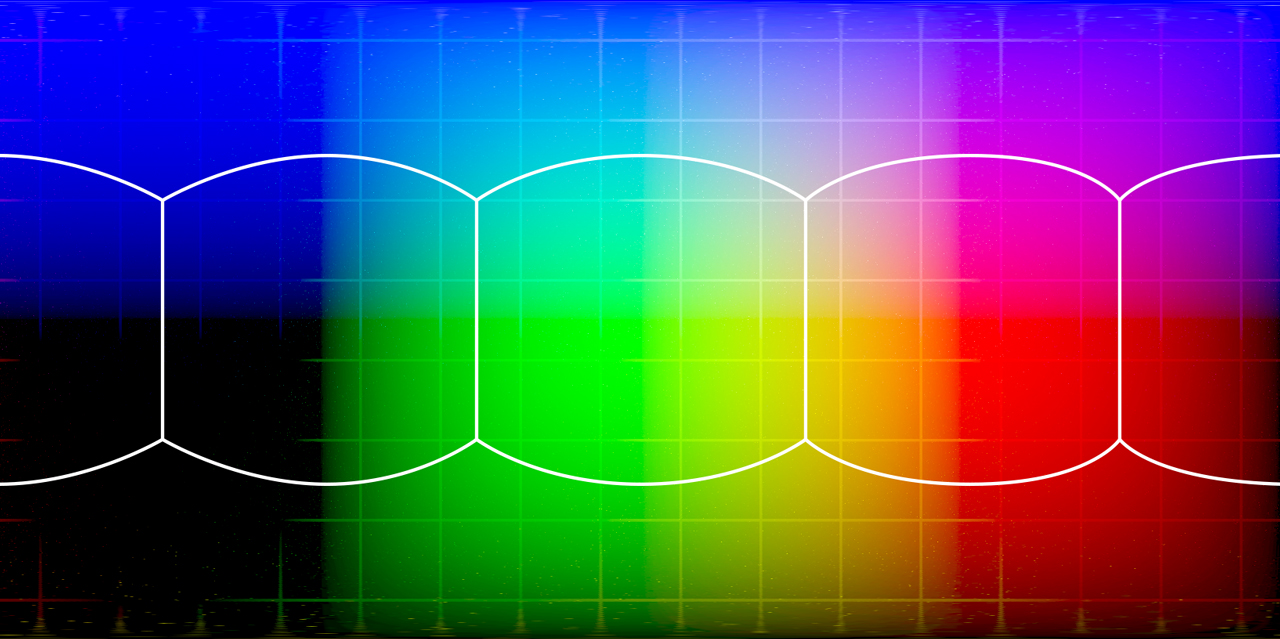
\includegraphics[width=3.0in]{../images/directioncubemap}
  \caption{A cube based directional map, overlaid with both lines of latitude and a cubemap adapted from \cite{EpicCube2016}.}
  \label{fig:cubemap}
\end{figure}

\section{Evaluation and Results}

Our first evaluation of the system was during a gesture elicitation study, where users navigated based on instructions (e.g., move left, move right, rotate, etc.), as shown in Figure~\ref{fig:expphoto}. The system performed successfully with the load of a multi-touch and Intel Real-Time sense camera. During the trials, we were able to constantly refresh the generated sky at 60 frames per second on an Nvidia 980 GTX \& 980m (circa 2014) with texels of 1024 pixels per cube face. On an Nvidia 650m (circa 2012) the effect was too taxing, running at 22 frames per second at 1024 texel size; however, 256 texel size ran smoothly at 60 frames per second.

\begin{figure}[bth]
  \centering
  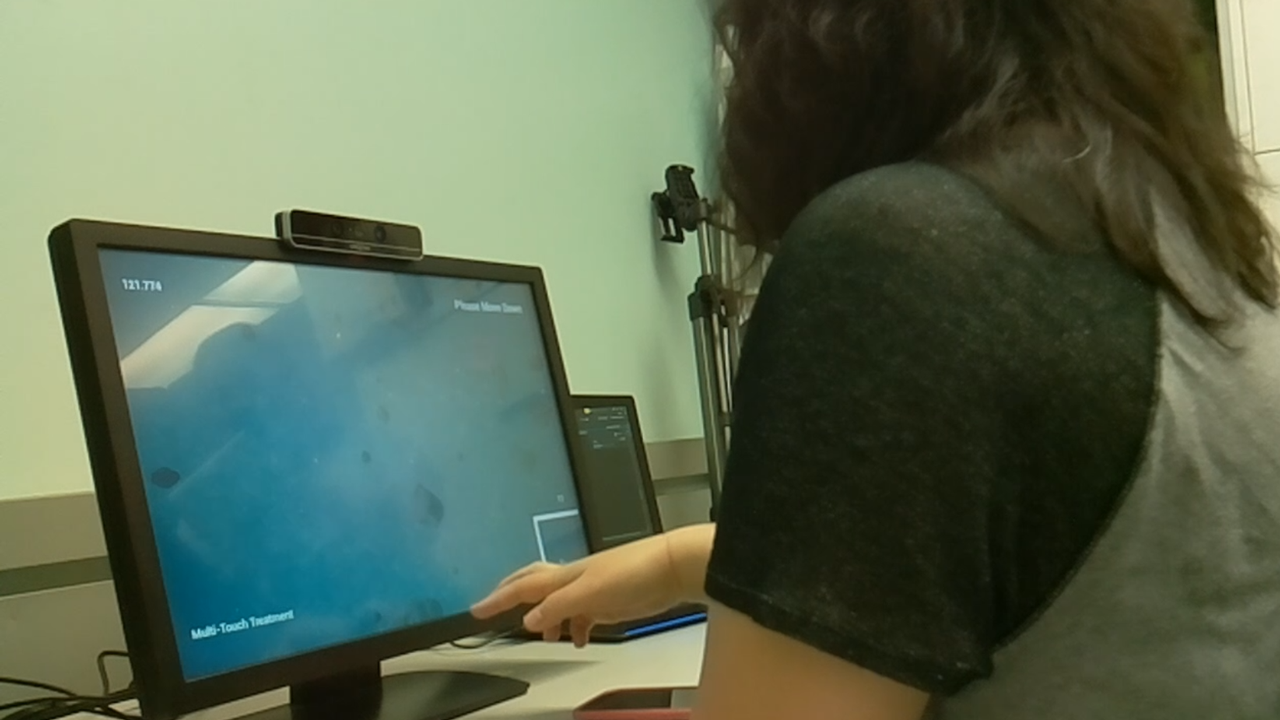
\includegraphics[width=3.0in]{../images/experiment-photo}
  \caption{Participant using Celestial Sky}
  \label{fig:expphoto}
\end{figure}
\section{Conclusions and Future Work}



We have presented a method for a physically-based, real-time rendering of celestial skies, building off of work from \cite{Jensen:2001fr}. Our approach provides other researchers with the ability to create large expanses of space for user interaction, in particular 3D navigation. Our method results in a celestial environment that is easier to manipulate in situations where the sky transforms, such as in a space ship or speeding up time. In addition, the use of cubemap lighting that looks similar to color corrected photographs provided by NASA provides an optional light source for dim environments such as night time.

In the future, we would like to provide a Vulkan implementation of the algorithm to compare performance with directX devices as well as to further optimize the algorithm by taking advantage of CPU concurrency on each face of the cubemap.  


% \section*{Acknowledgments}

% Special thanks goes to Wei Zeng for her insightful feedback. Thanks also to Ruben Balcazar and Mario Sanchez for their review. The distance fog used as a circumstellar disk is provided by Epic Games. This work was funded under FIU's High Performance Database Research Center's OpenHID Lab.



\bibliographystyle{abbrv}
%%use following if all content of bibtex file should be shown
%\nocite{*}
\bibliography{paper}
\end{document}
